\begin{comment}
	A Felhasználói dokumentáció tartalmazza
	- a megoldott probléma rövid megfogalmazását,
	- a felhasznált módszerek rövid leírását,
	- a program használatához szükséges összes információt

	Magába foglalja a telepítési- (vagy üzemeltetési-) és a végfelhasználói leírást. Ezek
	meghatározott célközönséghez szólnak, könnyen és gyorsan kell, hogy eligazítsák a
	felhasználót a program használatában!

\end{comment}

\section{Bevezetés}
%% A feladat rövid ismertetése (mire való a szoftver)
%% Célközönség (kik, mikor, mire használhatják a programot)
\section{Telepítési útmutató}
\subsection{Rendszer követelmények}
%% A rendszer használatához szükséges minimális, illetve optimális HW/SW környezet
	A program tesztelése Linux Mint 17.1 'Rebecca' Cinnamon 64-bit-es konfigurációjú gépen történt.
	\begin{center}
  	\begin{tabular}{| p{5cm} | p{8cm} |} 
  	\hline
        Operációs rendszer & debian alapú rendszer (ubuntu, mint)
    \\ \hline
        Apache & 2.4.7 (Ubuntu)
    \\ \hline
        Erlang & 5.10.4 emulator \newline (SMP,ASYNC\_THREADS) (BEAM)
    \\ \hline
        g++ & 4.8.2 (Ubuntu)
    \\ \hline
        Mozilla Firefox & 37.0.2
    \\ \hline
    
    \end{tabular}
    \end{center}

    Verzió telepítések ajánlott módja terminálból:
	\begin{verbatim}
	sudo apt-get update

	sudo apt-get install g++-4.8
	sudo update-alternatives 
	    --install /usr/bin/g++ g++ /usr/bin/g++-4.8 20
	sudo apt-get install erlang

	sudo apt-get upgrade
	\end{verbatim}
	Apache szerver konfigurációt elég csak a szerver gépen futtatni, a segéd számító gépeken nem szükséges, ezért a telepítést is csak ott szükséges elvégezni.
	\begin{verbatim}
	sudo apt-get install apache2
	sudo apt-get install libapache2-mod-proxy-html
	sudo apt-get install libxml2-dev
	\end{verbatim}
	A weboldal megtekintéséhez Mozilla Firefox javasolt, ennek azon a gépen kell működnie amelyiken a klienst kívánjuk futtatni.
\subsection{Rendszer konfiguráció}
Első lépésként a forráskódat másoljuk át a gépre.
Terminálban menjünk a mappába.
\begin{verbatim}
user@computername:[project](master)
\end{verbatim}

Az apache szerverhez kapcsolódó lépéseket csak a szerveren kell elvégezni.
\subsubsection{Apache szerver - szakdoli.config}
	A projektben található \texttt{/project/ServerConfig/szakdoli.conf} fájl mintájára létre lehet hozni a saját szerver konfigurációs fájlunkat.
	\newline
	Az elején megadjuk a külső figyelési pontot.
	\begin{verbatim}
	Listen 8086
	<VirtualHost *:8086>
	\end{verbatim}

	Beállíthatjuk a szerver admin-ját.
	
	\begin{verbatim}
	ServerAdmin webmaster@localhost
	\end{verbatim}

	A mappa helyét \textbf{mindenképpen módosítani kell} a projekt aktuális mappájára, ahova másoltuk.
	DocumentRoot és a Directory után is.
	
	\begin{verbatim}
		DocumentRoot /home/../project/WebPage/
		<Directory /home/../project/WebPage/>
	\end{verbatim}
	
	A szerver elosztott része a 8082 porton van elindítva, és erre hozunk létre egy proxy-t, hogy a weboldallal lehetősége legyen kommunikálni.
	
	\begin{verbatim}
		ProxyPass /API http://localhost:8082
		ProxyPassReverse /API http://localhost:8082
		<Proxy *>
		    Order deny,allow
		    Deny from all
		    Allow from all
		</Proxy> 
	\end{verbatim}
	
	Ha valami hiba van a szerveren, a logok segítségével ki lehet deríteni a hiba okát. Ehhez lehetőség van beállítani saját mappát is.

	\begin{verbatim}
		ErrorLog ${APACHE_LOG_DIR}/error.log
		CustomLog ${APACHE_LOG_DIR}/access.log combined
	\end{verbatim}

\subsubsection{Apache szerver - elindítás}
	Az előbbi pontban megvalósított szerver konfigurációs fájt át kell helyezni az \\ \texttt{apache2/sites-available} mappájába, és fel kell venni a konfigurálandó fájlok közé. Ha nincsen még a mód proxy\_http-re állítva, azt is meg kell csinálni az újraindítás (restart) előtt. 
	\begin{verbatim}
		sudo cp ./ServerConfig/szakdoli.conf 
		     /etc/apache2/sites-available/szakdoli.conf
		sudo a2enmod proxy proxy_http
		sudo a2ensite szakdoli.conf
	\end{verbatim}
	Ezután ha a fájl rendben van el lehet indítani a szervert, mely ezután figyelni fogja az adott portokat.
	\begin{verbatim}
		sudo /etc/init.d/apache2 restart
	\end{verbatim}

\subsubsection{Elosztott számításhoz}
	Ezt a folyamatot a szerveren és a segéd számításokat végző gépeken is el kell végezni. \newline
	Az Erlang node-ok kommunikációjához be kell állítani a \texttt{.erlang.cookie} fájlt mely a \texttt{/home}-ban található. 
	Nem biztos, hogy a fájlnak van írás joga. Ha nincs akkor adni kell neki, és meg kell nyitni valamilyen szerkesztőben.
	Szerkesztés után pedig ajánlott visszaadni az eredeti jogait.
	\begin{verbatim}
		sudo chmod +w ~/.erlang.cookie
		sudo vim ~/.erlang.cookie
		sudo chmod 400 ~/.erlang.cookie
	\end{verbatim}
	Az alábbi atomot tartalmaznia kell a fájlnak.
	\begin{verbatim}
		cat ~/.erlang.cookie
		distributed_interpolation_bylexy
	\end{verbatim}
	Ezután az Erlang-node-ok tudnak egymással kommunikálni, akár több gépen is.

\subsubsection{Szerver tesztelése}
	Az első üzembe helyezés előtt érdemes lefordítani a fájlokat, és lefuttatni a teszteket, hogy tudjuk hogy az Erlang és a C++ verzió kompatibilis az eredetivel. \newline
	A \texttt{/bin} mappában található fájlok segítenek minket a rendszer élesítésében, tehát ebben a mappában van lehetőség a futtatásra.  
	\begin{verbatim}
		$ cd project/bin/
	\end{verbatim}

	Először indítsuk el az alábbi fájlt, mely lefordítja nekünk a kellő részeket. Ennek a fájlnak a futása pár percet igénybe vehet. Ha nem sikerül lefutnia hiba nélkül, akkor nagy valószínűséggel az elosztott számítás nem konfigurálható. 
	\begin{verbatim}
		./setup.sh
	\end{verbatim}
	Ha sikeres volt a futás akkor elindíthatjuk az Erlang shell-t, és a \texttt{run.erl} fájl segítségével betölthetjük a lefordított elemeket. A \texttt{run:load()} futtatását shell indítás után egyszer szabad lefuttatni, mivel a NIF fájlok nem tudnak újra betöltődni, és ez hibát generál.\newline
	Érdemes ismét lefuttatni a teszteket, ha sikeres volt akkor a gép alkalmas arra hogy szerver vagy segéd gép legyen.
	\begin{verbatim}
		erl
		c(run).
		run:load().
		run:test().
	\end{verbatim}
	Ha az Erlang fájlokban módosítunk valamit akkor elegendő csak újraindítani a shell-t és lefuttatni a betöltés előtt az Erlang fájlok újrafordítását.
	\begin{verbatim}
		erl
		c(run).
		run:compile().
		run:load().
		run:test().
	\end{verbatim}  
	
%% Első üzembe helyezés leírása – ha van ilyen –, a program indítása (kivéve, ha nem egy
%%önálló alkalmazásról, hanem egy meglévő rendszer új komponenséről van szó). Itt
%%ellenőrizzük, hogy a telepítési útmutató megfelel-e a valóságos telepítési folyamatnak.

\subsection{Használati útmutató}
\subsubsection{Szerver elindítása}
	A szerver elindítását szintén a \texttt{/project/bin} mappában kell végezni. Miután az előző lépésben már a teszteket elvégeztük így elindíthatjuk a szervert és a gépeket.
	Adnunk kell egy nevet a node-unknak, melyet a shell indításakor az \texttt{-sname} kapcsolóval lehet megadni.
	\begin{verbatim}
		$ cd project/bin/
		erl -s toolbar -sname nodeNameForInterpolation
		c(run).
		run:load().
		run:test().
	\end{verbatim}
	Ha a shell-ben minden megfelelően működik (fájlok lefordultak, tesztek lefutottak) akkor inicializálhatjuk a portokat, a \texttt{run:initServer()} függvényével. Ez a függvény létrehozza a szerver és a node-figyelő folyamatokat. Kiírja nekünk a képernyőre a figyelő folyamat pid-jét mellyel lehetőségünk van tesztelni, amikor esetleg egy gép felcsatlakozik. 
	\begin{verbatim}
		(test@computername)4> node().
		test@computername

		(test@computername)5> run:initServer().
		WatcherNode : <0.100.0>
		...
	\end{verbatim}
	A számító folyamathoz szükségünk van a másik gépen meghívott \texttt{node()} eredményére, mivel ez a node inicializációjának paramétere. 
	\begin{verbatim}
		(test2@computername2)5> 
		    run:initNode(test@computername).
		<0.66.0>
	\end{verbatim}
	Ekkor ha sikeres volt a feliratkozás akkor a szerver gépen láthatjuk kiírva.
	\begin{verbatim}
		Worker Writed <10214.66.0> 'test2@computername2'
	\end{verbatim}
	A szerveren ezután le lehet futtatni esetleg többször is a tesztet, hogy tudjuk a közös kommunikáció és a tényleges szétosztás is megtörténik.
	\begin{verbatim}
		(test@computername)21> run:test(pid(0,100,0)).
		(test@computername)21> nodeHandler:getNodelist(pid(0,100,0)).
	\end{verbatim}
	Mivel a szerver portjai inicializálódtak, ezért a weboldalról is lehet küldeni a számításokat. 
	A weboldal elérhető az apache által megadott porton (8086). A weboldal elérhetővé vált az apache konfiguráció után, és a kommunikáció is működik, ha a szervert inicializáltuk. Az oldal Mozilla Firefox-ban lett tesztelve.
	\newline A hivatkozási link az alábbi formában elérhető, ahol <inet addr> a szerver gép ip-címe, vagy domain neve (például helyi gép esetén: localhost):  
	\begin{verbatim}
	http://<inet addr>:8086
	\end{verbatim}
	Közvetlen szerver kommunikációt az alábbi linken lehet elérni. 
	Ha a kommunikáció kiépül akkor az alábbi JSON-t kapunk válaszul, ha nem épül ki kapcsolat, akkor más hibaüzenetet kapunk. 
	\begin{verbatim}
	http://<inet addr>:8086/API 
	{"success":"false","msg":"Invalid Response"}
	\end{verbatim}
	A kliens-szerver kommunikációt még bonyolítja az elosztott kommunikáció.
	Mivel igen sok rendszert érint, a telepítési folyamat nem is biztos hogy minden gépen végig tud menni. \newline
	Viszont kellőképpen tesztelt a folyamat ahhoz hogy a felhasználó tudja már a telepítés után hogy a rendszerén működni fognak-e a számítások.
\subsubsection{Weboldal használata}
	A weboldalt a szerver konfiguráció után el lehet érni az \texttt{http://<inet addr>:8086} linken.

	\paragraph{}
	Amikor megnyitjuk az oldalt látjuk jobb oldalt a listát, bal oldalt pedig a Grafikon és Táblázat elnevezéssel az interpoláció szerkesztésére alkalmas felületet
	(Lásd: \ref{fig:webpage1}. ábra).

	\begin{figure}[h]
		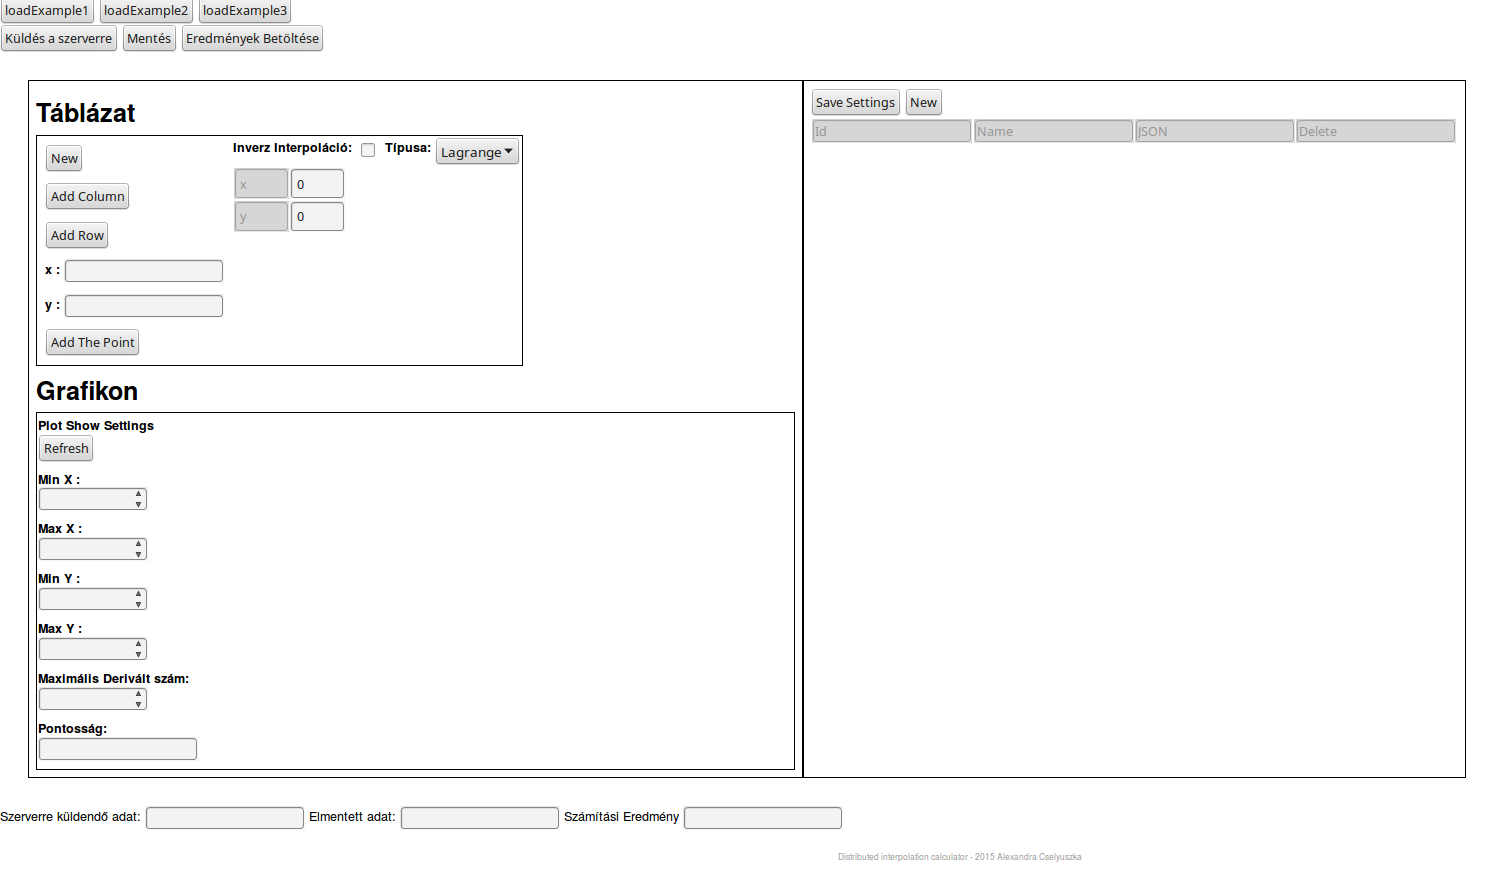
\includegraphics[width=15cm]{pics/webpage1}
		\centering
		\caption{Weboldal megnyitás után\label{fig:webpage1}}
	\end{figure}

	\paragraph{}
	Először a jobb oldalon található listában van lehetőségünk felvenni az interpolálni kívánt adathalmazokat. Egy sor egy interpolációs számítást jelent. Az sorban található gombra vagy szövegdobozokba kattintunk akkor az adott sor elemeit betölti.
	A \textit{"-- Törlés --"} gomb hatására viszont az adott sor törlésre kerül. \newline
	Adatok oszlopban látható az a json, amelyben az adatok el vannak tárolva egyesével. Ebből tölti be a bal oldalra az interpoláció pontjait és tulajdonságait is. A névre kattintás hatására az adatok abból a sorból betöltődnek (Lásd: \ref{fig:webpage_menulist}. ábra). \newline 
	A listába van lehetőségünk kívülről is betölteni adatokat. Például ha frissítjük az oldalt a lista kiürül, de az utoljára felvett értékeket az \textit{"Elmentett adat"} JSON-jében megtalálhatjuk, és onnan az \textit{"Eredmény betöltése"} gombbal van lehetőségünk betölteni a listába.

	\begin{figure}[h]
		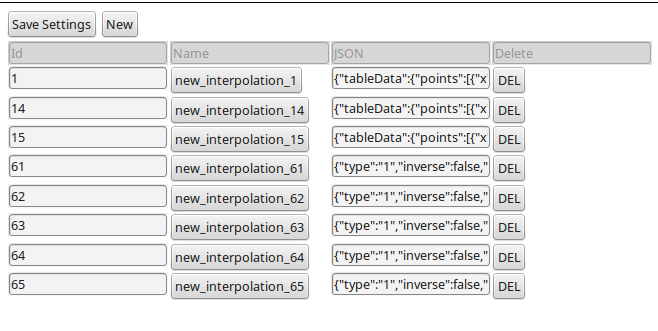
\includegraphics[width=11cm]{pics/webpage_menulist}
		\centering
		\caption{Interpolációk listája\label{fig:webpage_menulist}}
	\end{figure}
	
	\paragraph{}
	Ha kiválasztottuk a sort, akkor megjelenik a bal oldalon a grafikon és a táblázat az aktuális értékekkel. A táblázatba felvehetünk új pontokat, és azokat a frissítés gomb hatására a grafikonon is megtekinthetjük. A grafikonon kattintva az aktuális koordináták bekerülnek az x,y elnevezésű inputokba, ahonnan a \textit{"Pont hozzáadása"} gomb segítségével bekerül a táblázatba (Lásd: \ref{fig:webpage_table_plot}. ábra). Mielőtt az új pontot felvennénk, kézzel is szerkeszthetjük. A táblázatban van lehetőség új oszlopok és sorok felvételére, és az egyes pontok szerkesztésére. Miután a pontokat kézzel szerkesztettük a grafikon mellett található \textit{"Frissítés"} gombbal a grafikonon is megtekinthetjük.

	\begin{figure}[h]
		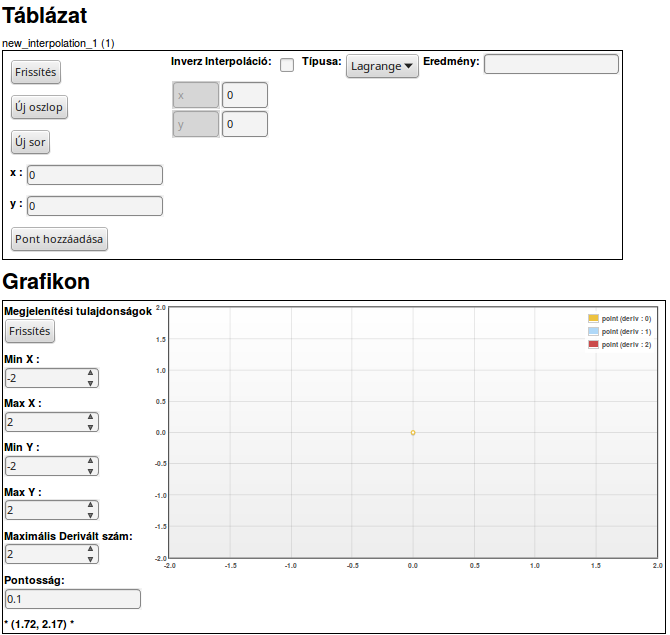
\includegraphics[width=15cm]{pics/webpage_table_plot}
		\centering
		\caption{Grafikon és táblázat\label{fig:webpage_table_plot}}
	\end{figure}

	\paragraph{}
	Az oldalon megtekinthetőek még az egyes részekhez tartozó gombok, melyekkel új elemeket lehet létrehozni, vagy törölni régieket, valamint van lehetőség a mentésre is (Lásd: \ref{fig:webpage_buttons}. ábra).
	A \textit{"Minta 1"} gomb segítségével minta adathalmazt lehet betölteni a \textit{"Elmentett adat"}-ba, majd onnan az \textit{"Eredmény Betöltése"} gombbal a listában is megtekinthetjük. 
	\newline Ha befejeztük az adathalmazok szerkesztését akkor a küldés gombbal van lehetőség a szervernek elküldeni a szerkesztett adatokat.
	\newline 
	A szerver számítás után felugrik egy ablak, amelyben megkapjuk válaszul hogy sikeres vagy sikertelen volt a szerver kommunikáció (Lásd: \ref{fig:webpage_unsuccess}. ábra). 
	\newline
	A sikeres kommunikáció ablakában megtekinthető a számítás ideje is, mely csak a szerveren számított időt méri, a szerver és a kliens közötti kommunikáció ezt az időt nem befolyásolja. \newline
	Sikeres szerver kommunikáció esetén ha a listában kiválasztunk egy elemet, akkor annak eredményét is megtekinthetjük, a grafikonon.
	\newline Abban az esetben amikor szerver hiba van nagy valószínűséggel a szerver kapcsolatban van a gond. Első lépésként ellenőrizni kell a szervert, hogy működik-e, és a tesztjei lefutnak-e. Ha működik minden tesztje és fut a szerver, mégis hiba van akkor az adatforgalmat kell ellenőrizni, hogy minden információ megérkezett-e, érdemes ilyenkor a szerver kommunikációt kielemezni, nincs-e valami korlátozva, vagy blokkolva.
	\newpage
	Ha számítás sikeres volt akkor az interpoláció kiválasztása után megtekinthető lesz az eredmény. Ha nem sikerült az adott interpolációhoz a számítást végrehajtani, akkor nem láthatjuk a polinomot, és a szerveren az Erlang shell-ben megjelenik nagy valószínűséggel a hibaüzenet.

	A feladat felületi oldala egyszerűen átlátható, de a gombok és listák kezelése nem kellőképpen dinamikus. Ennek az is az oka hogy egy elég komplex felületről van szó, ahol minden egységnek minden egységgel kommunikálnia kell valamilyen formában. \newline
	Az adatok szerkesztése után egy gombra kattintással el is küldi a szervernek a szükséges információkat, melyekből a szerver számol, és eredményt ad vissza. \newline
	Ha minden sikeresen végre hajtódik, akkor a felhasználó a kívánt ponthalmazokat és polinomokat láthatja a grafikonon, mint a sikeres interpoláció eredményét.

	\begin{figure}[h]
		
\includegraphics[width=7cm]{pics/webpage_buttons}
		\centering
		\caption{Globális gombok\label{fig:webpage_buttons}}
	\end{figure}

	\begin{figure}[h]
		
\includegraphics[width=15cm]{pics/webpage_inputs}
		\centering
		\caption{Adatok betöltése, mentése az inputokba történik \label{fig:webpage_inputs}}
	\end{figure}

	\begin{figure}[h]
		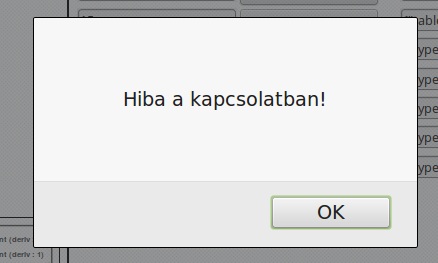
\includegraphics[width=6cm]{pics/webpage_unsuccess}
		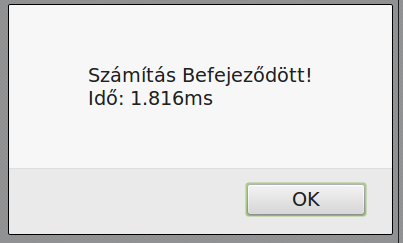
\includegraphics[width=6cm]{pics/webpage_success}
		\centering
		\caption{Sikeres és sikertelen kapcsolat\label{fig:webpage_unsuccess}}
	\end{figure}

	\begin{figure}[h]
		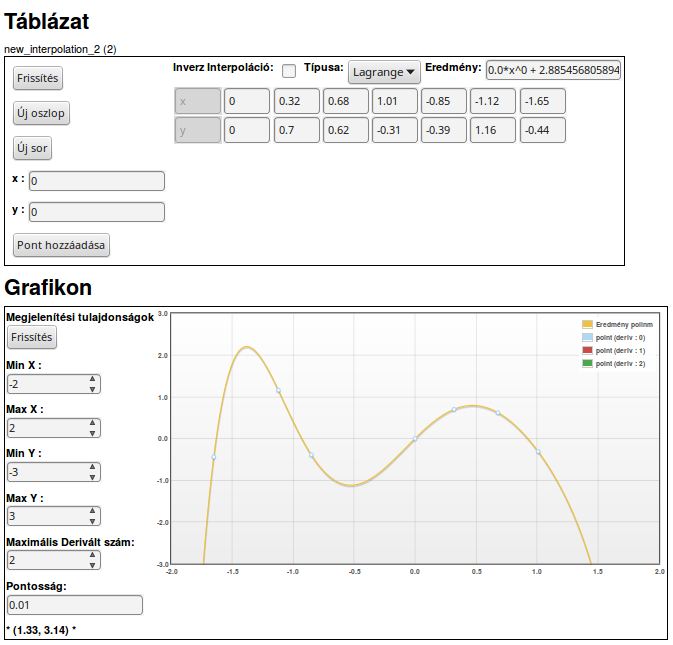
\includegraphics[width=14cm]{pics/webpage_plot_result}
		\centering
		\caption{Eredmény kirajzolása\label{fig:webpage_plot_result}}
	\end{figure}

%% Általános felhasználói tájékoztató (például a szokásostól eltérő képernyő-, billentyű-,
%%illetve egérkezelés leírása, teendők hibaüzenetek esetén stb.).
%% A rendszer funkcióinak ismertetése. A feladat jellegéből fakadóan célszerű lehet ezt
%%folyamatszerűen, képernyőképekkel alátámasztva bemutatni. A funkciókat ajánlatos a
%%felhasználói szintek szerint csoportosítani. Itt vegyük figyelembe, hogy a leírás a
%%fejlesztői dokumentációban meghatározott részfeladathoz illeszkedik-e, az ott
%% meghatározott funkciókat/használati eseteket írja-e le?
%% A rendszer futás közbeni üzenetei (hibaüzenetek, figyelmeztető üzenetek, felszólító üze-
%%netek stb.) és azok magyarázata – az esetleges üzemeltetési teendőkkel együtt. Itt vegyük
%%figyelembe, hogy tartalmaz-e biztonsági, illetve hibaelhárítási előírásokat?
%% Egyéb, a szoftver használatához szükséges információk.
